\chapter{Hardware}

% What am I trying to say in this chapter:
% 1) OpenVGA PCB + IC overview.
%	- Diagram of PCB
%	- List of ICs, small description of function
%	- Trace impedance/signal integrity?
% (This could all end up in the intro)
% 2) IC Detail
%	- Selection criteria
%	- IC descriptions
% 3) PCB Detail
%	- Design considerations, placement+layer constraints
%	- Power distribution
%	- Parallel buses
%	- Signal integrity

OpenVGA hardware consists of a two-layer PCB, some connectors, decoupling and
terminating capacitors and resistors, and an FPGA and supporting ICs (see
Figure~\ref{OPENVGA_OpenVGA}). The PCB form-factor is a full-height, short,
PCI expansion board with rear I/O panel connectors. Factors which influenced the
PCB design and choice of components are cost, availability, and simplicity.

\begin{figure}[h!]
\begin{center}
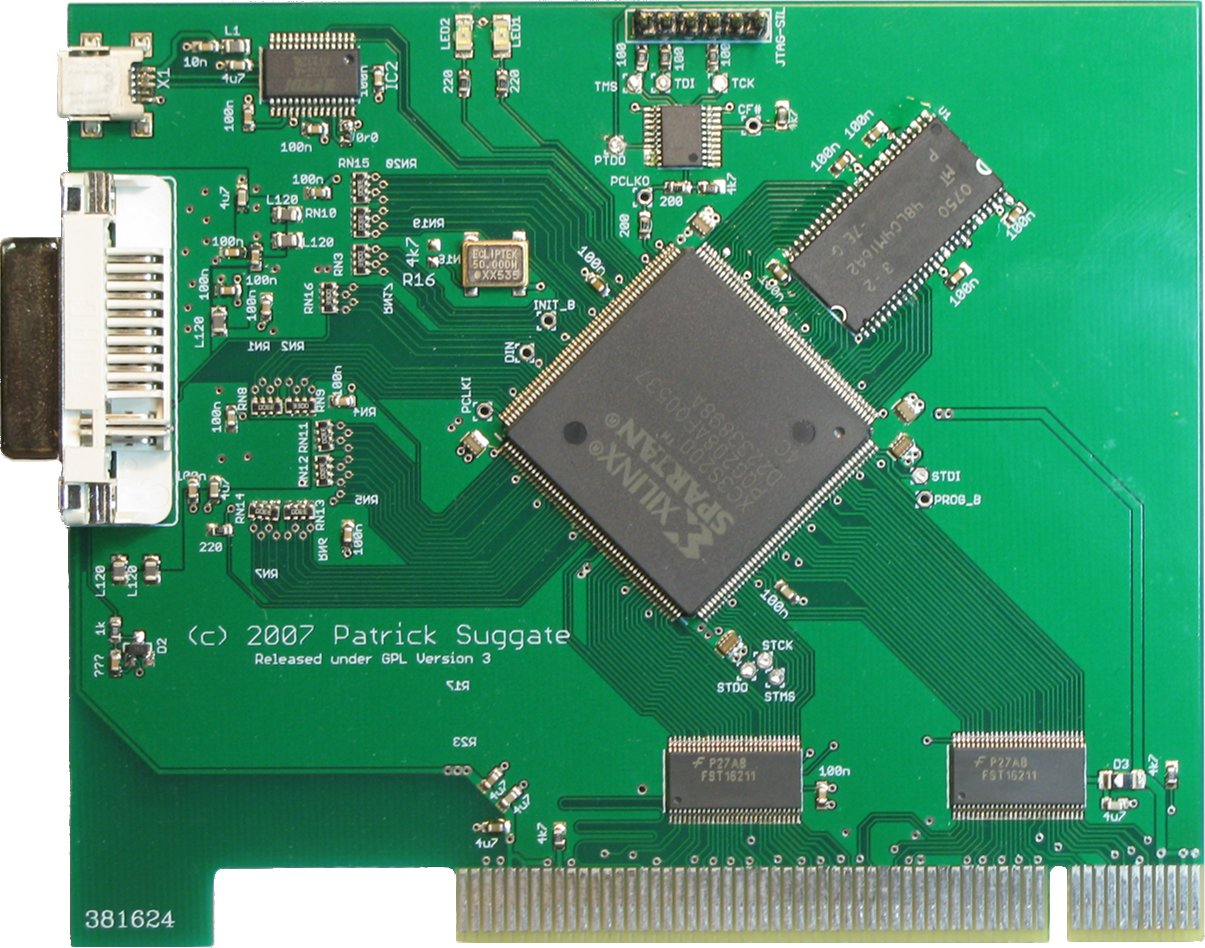
\includegraphics[width=\linewidth]{images/freega_overview.eps}
\caption[OpenVGA Hardware Summary]{OpenVGA Hardware Summary.}
\label{HARD_OpenVGA}
\end{center}
\end{figure}

% \begin{figure}[!h]
% \begin{center}
% \includegraphics[width=\linewidth]{diagrams/freega_simple.eps}
% \caption[PCI Stub Board]{Simplified diagram of the OpenVGA hardware.}
% \label{HARD_FreeGA_Simple}
% \end{center}
% \end{figure}


\section{Features and Components}
The core of OpenVGA is a FPGA which contains the logic necessary for implementing
a display device. This FPGA is a Xilinx Spartan-3, which is Xilinx's low-cost
product family, with a rated quantity of programmable logic equivalent to an IC
with about 200,000 gates. The complete OpenVGA HDL, when synthesised, only uses
about 60\% of this.

Display devices require a frame-buffer to store image data, and since the
internal memory capacity of the FPGA is only 246 k-bits, OpenVGA has an 8 MB SDRAM
IC, connected via a 16-bit data bus and operating at 100 MHz.

Driving VGA and DVI monitors is not possible with the chosen FPGA so the OpenVGA
board also features a DVI transmitter IC and a video DAC. These ICs can drive a
DVI and VGA display respectively. These are connected to the FPGA via parallel
buses, 12-bit DDR for DVI, and 24-bit for VGA.

Since the state of RAM based FPGAs is typically lost on
power-off\cite{Xilinx_SP3_DS}, a SPROM (Serial Programmable Read-Only Memory) is
used to restore the state at power-on. This is programmed via JTAG, like the
FPGA.

% TODO

Both the VGA and DVI output signals of OpenVGA cannot be generated by the Spartan
III so a video DAC was used for the VGA output signal, and a TMDS
(Transition-Minimised Differential Signalling) encoder was used for DVI.

\begin{table}[h!]
\begin{center}
\begin{tabular}{l | r | l}
Name				& Part\#		& Description	\\
\hline
Xilinx Spartan-3	& xc3s200-4	& FPGA	\\
Philips Video DAC	& tlp555	& Generates analogue VGA signals from \\
					&			& 24-bit digital RGB data \\
Bus switches		& 74c12345	& Bus transmitter ICs which perform voltage
translation	\\

\end{tabular}
\end{center}
\end{table}

% \section{FPGA Selection} When OpenVGA was first started, the available FPGAs
% from the three main vendors low-cost range were Spartan III(TM) from
% Xilinx(TM), Cyclone II(TM) from Altera(TM), and ECP2(TM) from Lattice Semi(TM).
%  Due to reasons of cost, performance, availability, and prior experience,
% Spartan III FPGAs were used.  \begin{tabular}{| l || l | l | l | l |} \hline
% FPGA Family & Speed & Size & Cost & Other \\
% \hline Spartan III & 200 MHz & 2-110k LEs & \$20 & Widely available, free
% GNU/Linux software tools
%  \\
% Cyclone II & 220 MHz & 3-90k LEs & \$30 & Harder to obtain, Free Windows-only
% tools \\ ECP2 & 220 MHz & 3-70k LEs & \$25 & Widely available, no free tools
% except trial versions \\
% \hline \end{tabular}
\subsection{FPGA}
The FPGA used is a 208 pin, quad flat pack, 200 kGate, Xilinx Spartan-3. This
FPGA is the central element of OpenVGA with all I/O peripherals and storage --
Video DAC, DVI TMDS transmitter, 8MB SDRAM IC, 4Mb SPROM, PCI bus switches, and
USB to serial IC -- connected to it.

The Spartan-3 IC requires at least two supply voltage rails, 1.2 V for the core
and 2.5 V for the I/O pins during configuration. Additionally, a 3.3 V supply was
needed to interface to the SDRAM, PCI bus switches, DVI transmitter, Video DAC,
and USB to serial IC.

With a two-layer PCB it is not possible to have a separate power plane for each
of the three supply voltages plus the supply ground. The already significant
number of required decoupling capacitors\cite{Xilinx_Decoupling} was increased to
preempt any grounding and power supply issues.

Most of the FPGA non-supply or ground pins are general purpose, but there are
some that are used for configuration. These dictated the most sensible layout for
the PCB since it was easiest to have the configuration serial PROM at the top of
the PCB, with its traces out of the way of the parallel interfaces of the other
ICs.

Another significant FPGA positioning constraint is caused by a side-effect of the
internal layout of the FPGA. The logic within the FPGA exhibits the highest
performance when the designs data-flow is East-West or West-East. Consequently,
the FPGA I/O banks on the East and West edges have the greatest number of I/O
pins available too. High speed devices would benefit from using these banks. The
highest speed device used for OpenVGA was the SDRAM IC, which also requires a high
number of FPGA I/O pins, so this was placed adjacent to the East bank of FPGA I/O
pins.


\subsection{SDRAM and DVI\ldots Termination}
OpenVGA's two-layer PCB means that the traces are quite far from the ground-plane,
compared to a four-layer PCB, so trace impedances are much higher than a four
layer board. These impedances were calculated using Transcalc, and using the
equation described by Wheeler\cite{wheeler1977mtt}.
\begin{equation}
Z_o	= \sqrt{H}
\end{equation}


\subsection{VGA DAC}
The video DAC takes the three video signal colour components, upto ten bits wide,
and a clock signal and produces analogue red, green, and blue outputs at voltage
level compatible with VGA (0.7V to 1.1V CHECK).



\subsection{DVI Transmitter}
The DVI TMDS has a similar interface as the video DAC but the encoder generates a
differential output clock that has 10 times the frequency of the input clock and
TMDS colour components running at this frequency. Each colour component
differential pair uses a 10-bit encoding scheme to encode the 8-bit per component
colour data. The purpose of the 10-bit encoding is to encode the data in such a
way that minimises the number of signal transitions between high and low signal
levels. This encoding increases signal inegrity which allows the signal to be
tranmitted over a long cable, with specifications requiring that the signal must
be able to be transmitted at least 5 metres, though cables can be shorter than
this.

\begin{figure}
\begin{center}
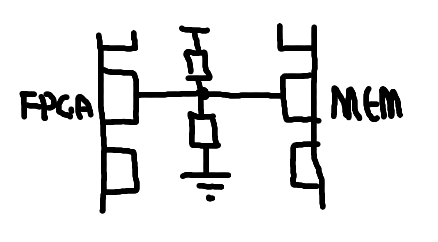
\includegraphics[width=\linewidth]{images/async_fifo.eps}
\caption{TMDS Encoding.}
\end{center}
\end{figure}




\subsection{PCI Bus Switches}
The PCI Local Bus uses half-wave reflection signalling\cite{PCI_Spec, PCI_Book}
which causes voltage transients that exceed the maximum operating conditions
specified for the Spartan III family\cite{Xilinx_SP3_DS}. Two 24 pin bus switches
were used to prevent PCI signals from exceeding 3.4 V and -0.7 V. These switches
add a propagation delay of 250 ps\cite{Bus_Switch_DS}.

\begin{figure}[h!]
\begin{center}
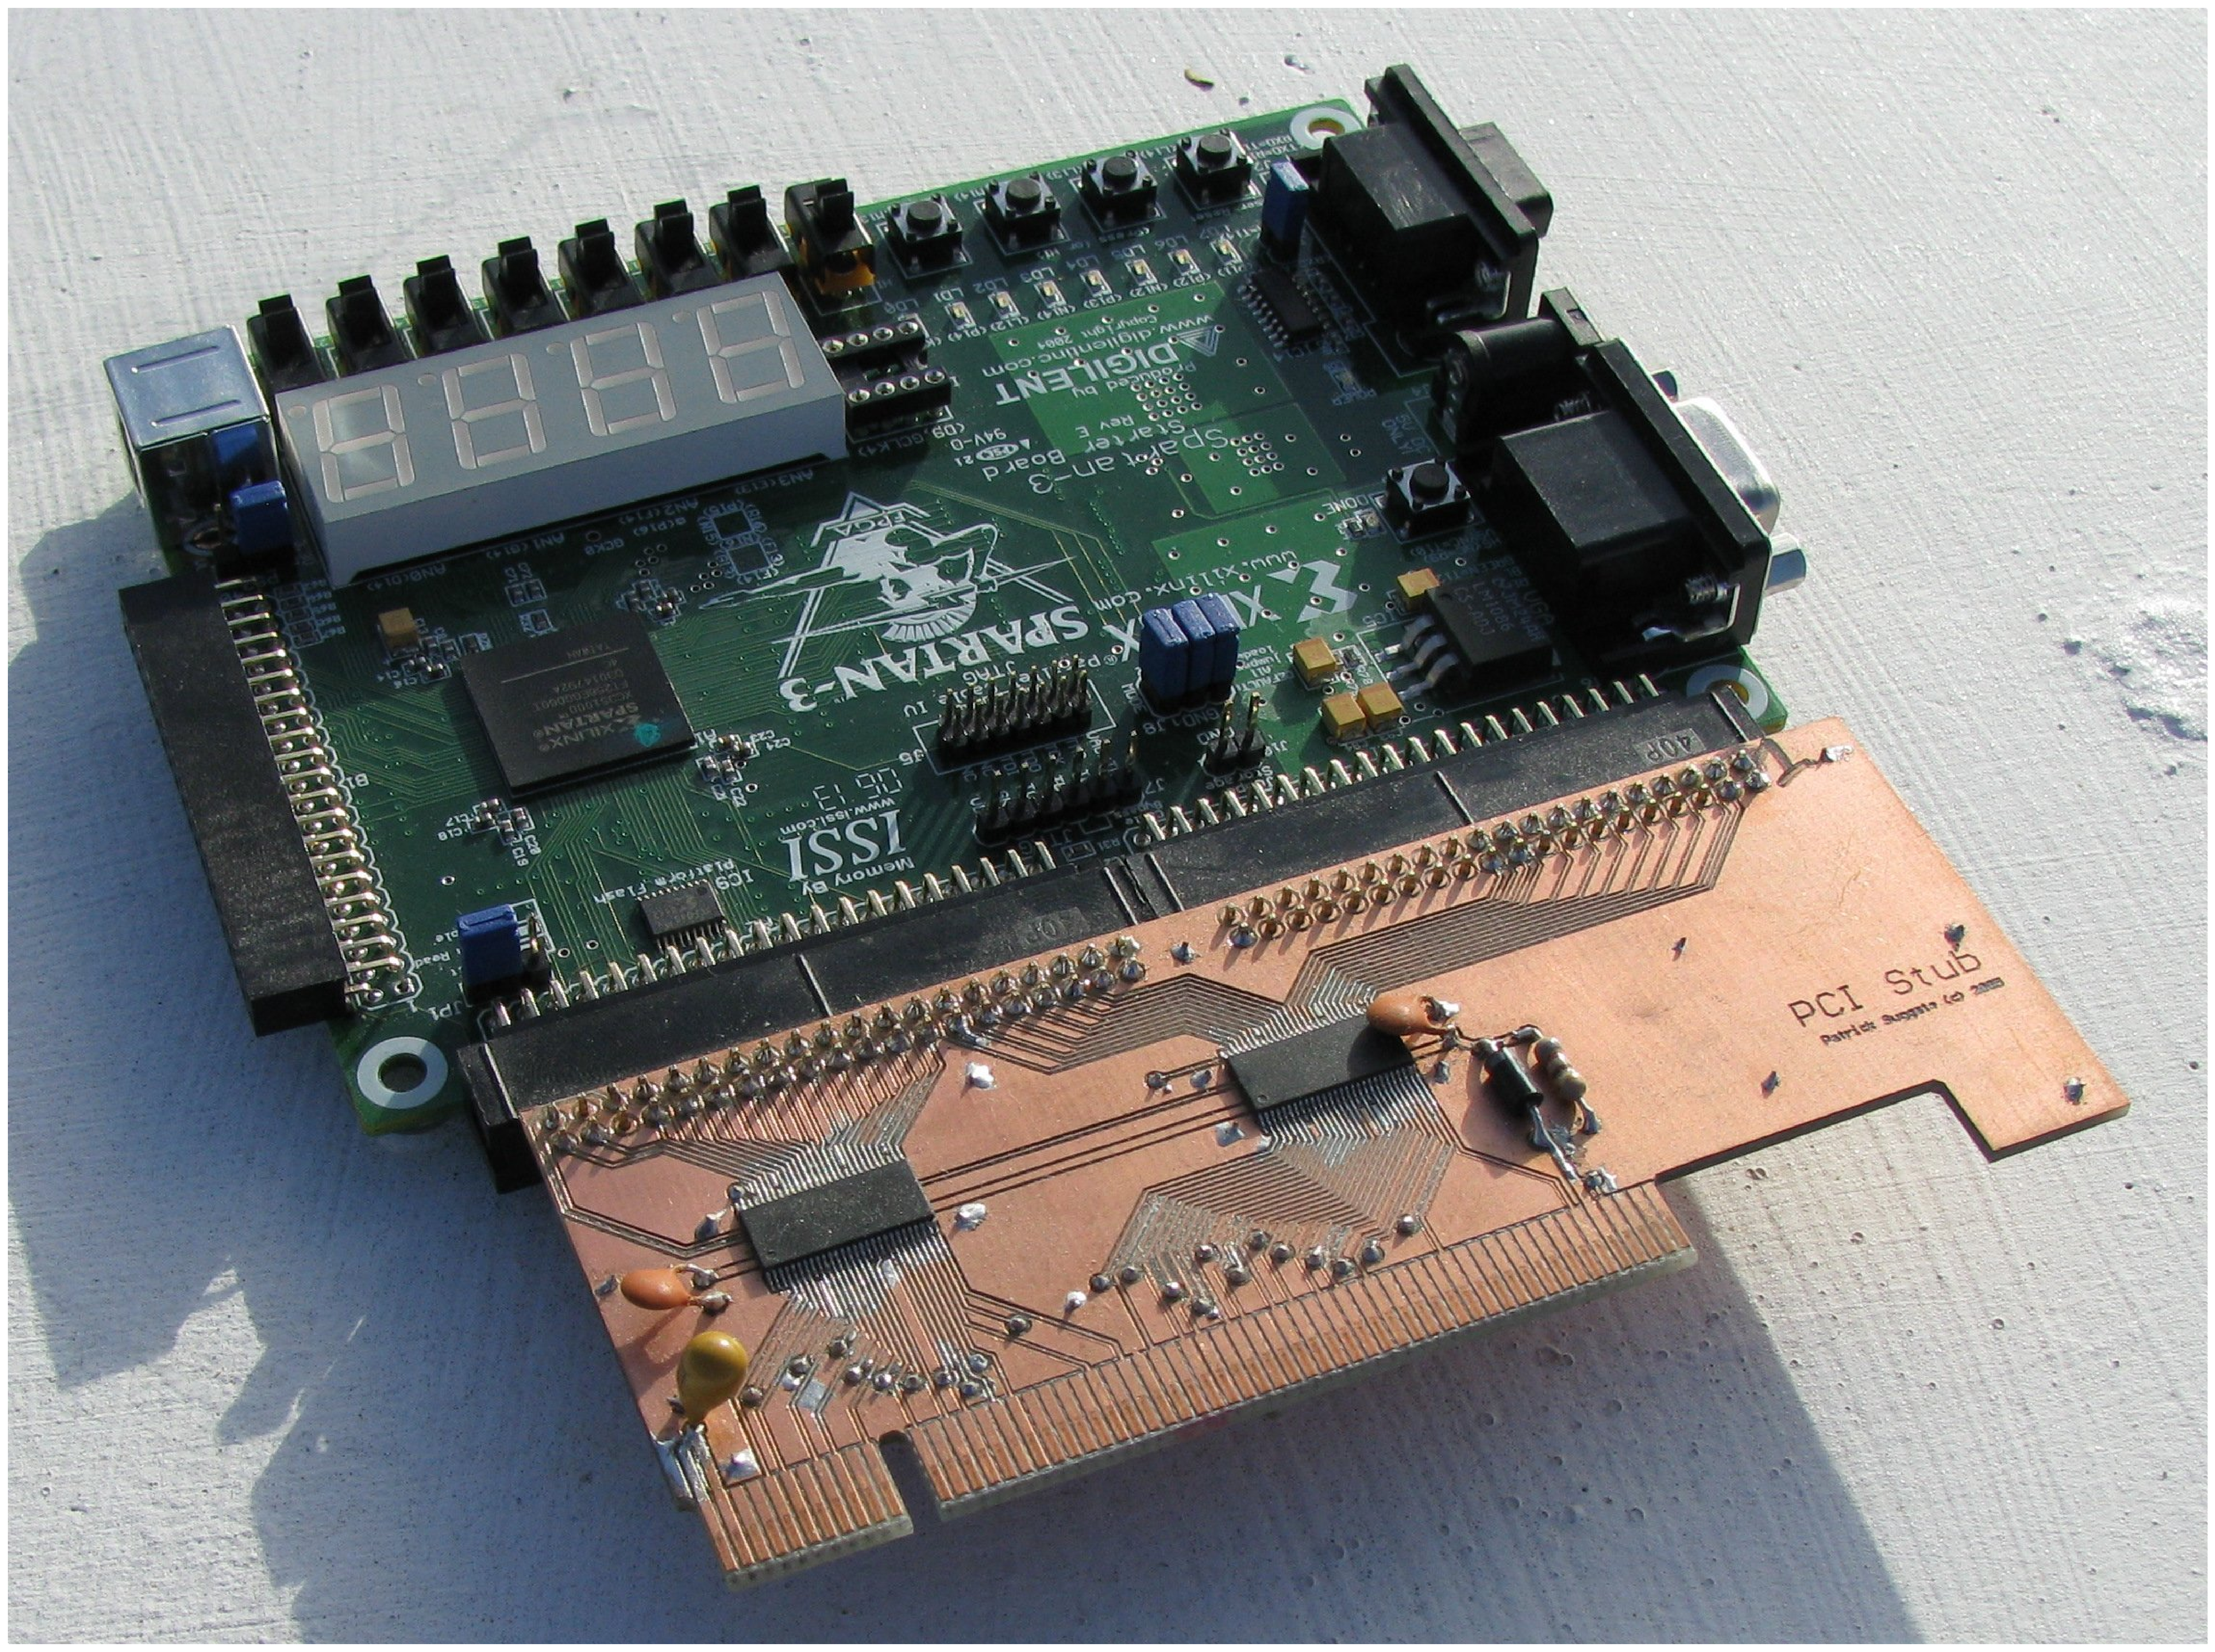
\includegraphics[width=\linewidth]{images/pci_stub.eps}
\caption[Stub board for PCI development]{Stub board for PCI development. The
bus-switches, which are visible in the middle of the copper coloured PCB,
translate the PCI's 5 V signals to 3.3 V required by the Spartan-3 FPGA.}
\end{center}
\end{figure}


\subsection{DDR SDRAM}
Architecturally, DDR SDRAM is very similar to SDRAM\cite{inc:mxx}, but two words
are fetched in parallel, with the first word being transmitted half a clock cycle
earlier than the second word, doubling the effective throughput.

For OpenVGA, DDR SDRAM was initially tried, on a two-layer PCB, but difficulty
with trace impedance matching and termination, meant that it never worked
correctly. Placement and routing of large numbers of termination resistors was
very difficult with a two-layer PCB.

\begin{figure}
\begin{center}
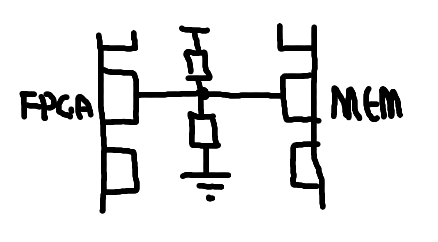
\includegraphics[width=\linewidth]{images/ddr_term.eps}
\caption{DDR SDRAM Termination Scheme.}
\end{center}
\end{figure}

\begin{figure}
\begin{center}
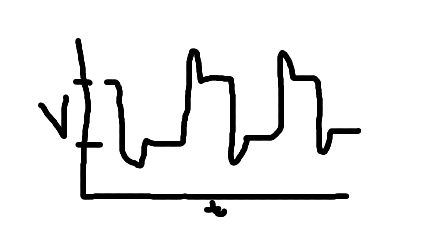
\includegraphics[width=\linewidth]{images/ddr_overshoot.eps}
\caption[Undershoot/Overshoot with DDR SDRAM]{Undershoot/Overshoot with DDR
SDRAM.}
\end{center}
\end{figure}



\section{PCB Detail}

\subsection{PCB Design}
The PCB was designed to be manufactured as a two-layer PCB, as this
significantly reduces manufacturing time, NRE (Non-Recurring Engineering)
charges as well as cost per inch of PCB\cite{Our_PCB}. Disadvantages of a two
layer PCB include increased routing complexity -- both signals and power supply
-- and poorer signal integrity compared to a four-layer, or more, PCB (see
Section~\ref{HARD_Signal_Integrity}).

There were three versions of the OpenVGA PCB (see Figures~\ref{HARD_PCI_Stub},
\ref{HARD_FreeGA_DDR}, and \ref{OPENVGA_Version2}). The first was to develop
stable PCI modules, the second was milled in-house to experiment with DDR SDRAM, and the
third was the final version with SDR SDRAM.

\begin{figure}
\begin{center}
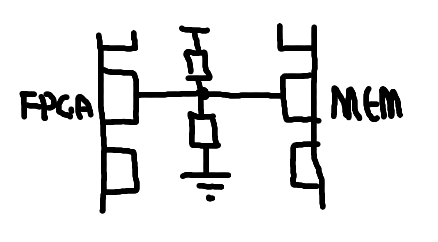
\includegraphics[width=\linewidth]{images/async_fifo.eps}
\caption[PCI Stub Board]{Initial OpenVGA version, simply a PCI header board
with voltage translators, and the VGA outputs were only eight colours.}
\label{HARD_PCI_Stub}
\end{center}
\end{figure}

\begin{figure}
\begin{center}
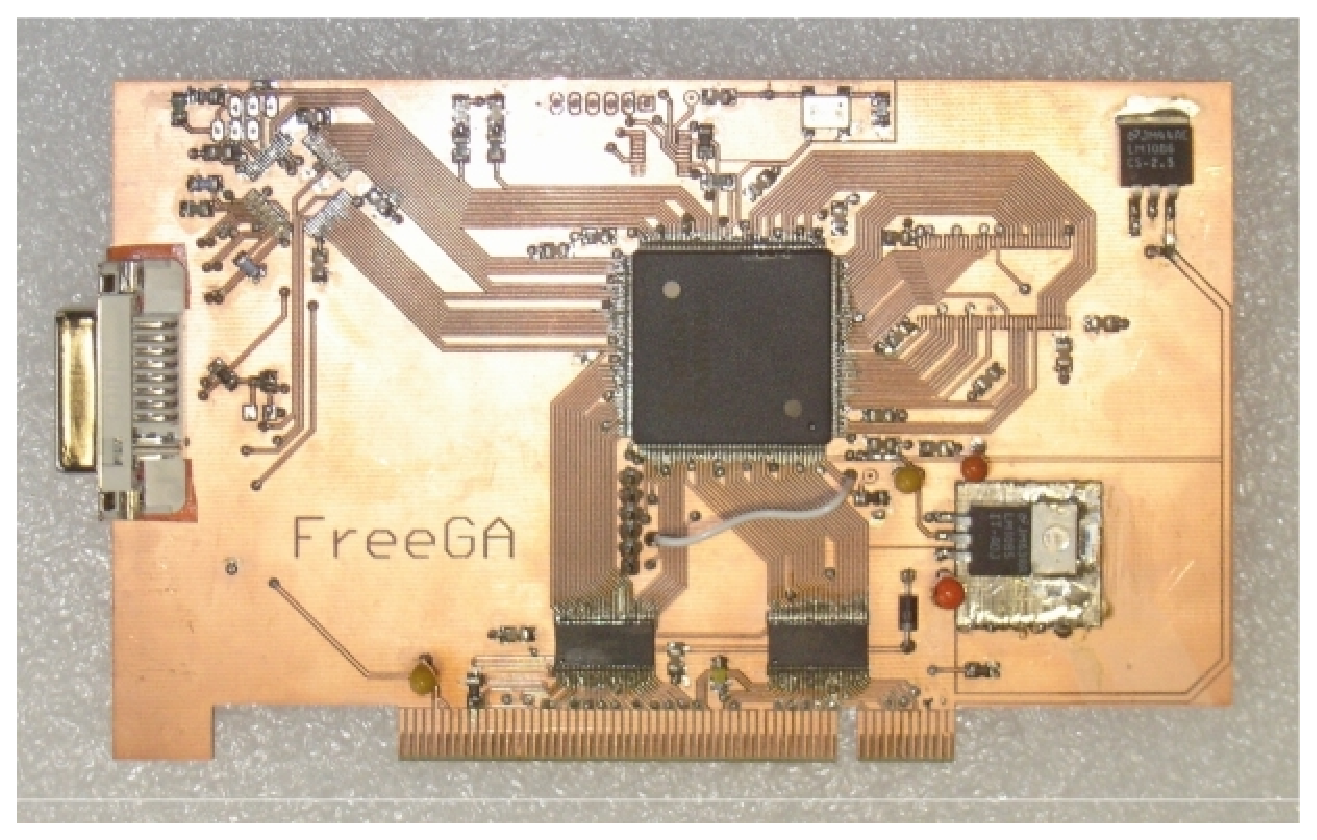
\includegraphics[width=\linewidth]{images/FreeGA_orig.eps}
\caption[OpenVGA V2 with DDR SDRAM]{Milled PCB featuring DDR SDRAM, DVI, and
only eight colour VGA (via the DVI analouge outputs).}
\label{HARD_FreeGA_DDR}
\end{center}
\end{figure}


\begin{figure}
\begin{center}
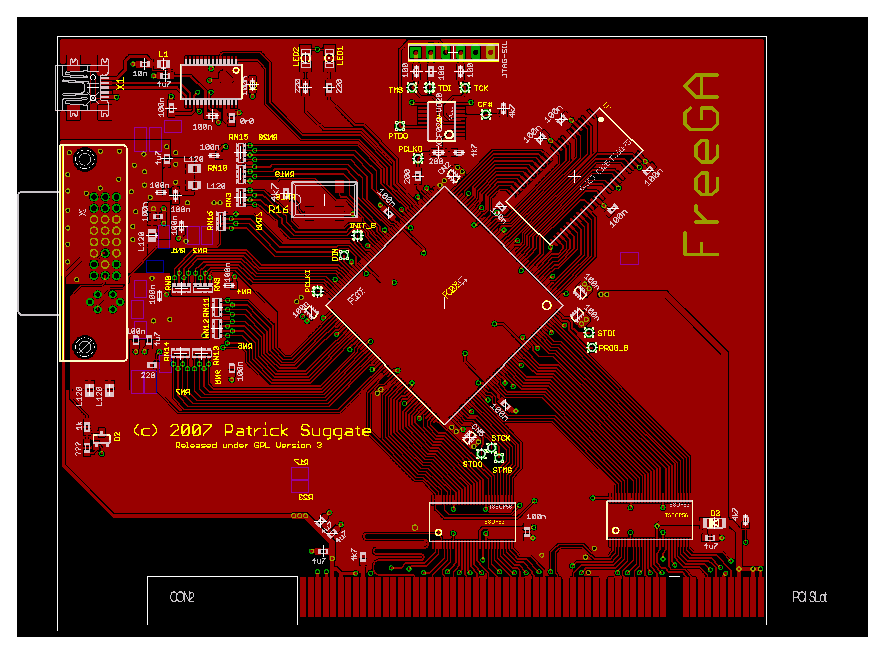
\includegraphics[width=\linewidth]{images/freega3_pcb_art_top.eps}
\caption[OpenVGA PCB Artwork Top Layer]{OpenVGA PCB artwork for the top layer.}
\end{center}
\end{figure}

\begin{figure}
\begin{center}
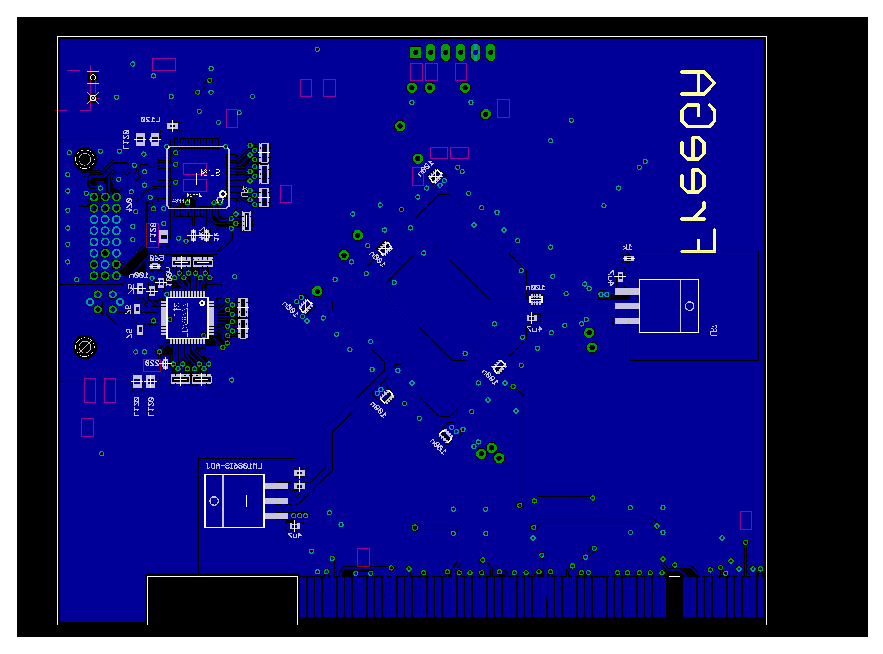
\includegraphics[width=\linewidth]{images/freega3_pcb_art_bot.eps}
\caption[OpenVGA PCB Artwork Bottom Layer]{OpenVGA PCB artwork for the bottom
layer.}
\end{center}
\end{figure}


\begin{figure}
\begin{center}
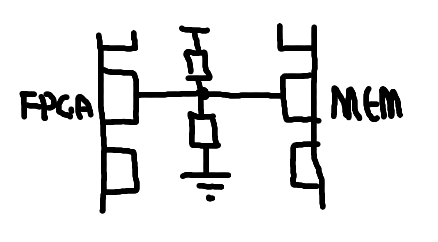
\includegraphics[width=\linewidth]{images/async_fifo.eps}
\caption[Differences between the geometry of two and four -layer
PCB]{Differences between the geometry of two and four layer
PCB. The four-layer PCB can have supply planes very close to the traces
improving signal integrity.}
\label{HARD_PCB_Comp}
\end{center}
\end{figure}


\subsection{Component Layout}
\begin{tabular}{l l}
\textbf{File:}			& FreeGA.brd	\\
\textbf{Description:}	& Maps a piece of local memory to the PCI Local Bus.\\ 
\textbf{Related Files:}	& /brd/FreeGA/FreeGA.sch, /brd/lib/xilinx.lbr	\\
						& /brd/lib/memory-samsung.lbr	\\
\end{tabular}

The components were laid out so with the goal of having the majority of the
signal routing on the top-side (the component-side) so that the bottom layer
could be used mostly for routing power supply and ground nets. The VGA and DVI
transmitter ICs were mounted on the solder layer, to simplify routing, and
decoupling capacitors and termination resistors were mounted on both sides of
the PCB.

The FPGA has mostly user assignable inputs and outputs so this allowed flexible
placement of most of the other ICs. Video transmitters could be near the back
edge and SDRAM could be placed so as to minimise trace lengths.

\subsection{Signal Integrity}
\label{HARD_Signal_Integrity}
OpenVGA drives and receives 150 high speed external digital signals. The PCI
signals operate at 33 MHz, the external oscillator at 50 MHz, the VGA and DVI signals
at upto 165 MHz, and the SDRAM signals at either 50 MHz or 100 MHz. For signals
above 25 MHz, careful design is needed to prevent signal integrity
problems\cite{HighSpeedDigitalDesign}. These can be ringing, crosstalk, and
issues arising from poor power supply and distribution.

\label{PCB_DDR}
DDR SDRAM.


\subsubsection{Reflections}
The highest frequency sections of the design, the connections between the
Spartan III and the VGA DAC, and the Spartan III to the DVI TMDS decoder, used
termination resistors matched to a $75\Omega$ trace impedance. An earlier
version of OpenVGA exhibited reflections causing peak voltages nearly twice that
of the driving voltage.

\begin{figure}
\begin{center}
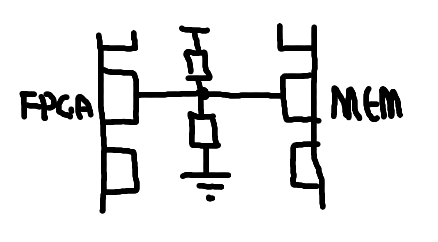
\includegraphics[width=\linewidth]{images/async_fifo.eps}
\caption[DDR signal showing reflections]{Trace showing reflections caused by
impedance mis-match.}
\end{center}
\end{figure}

\begin{figure}
\begin{center}
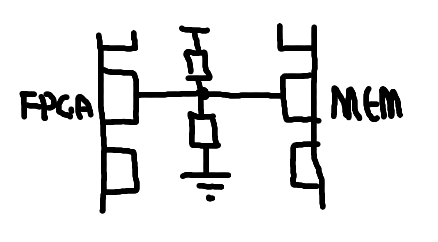
\includegraphics[width=\linewidth]{images/async_fifo.eps}
\caption[Terminated DDR signal without reflections]{Trace showing no reflections
due to effective signal termination.}
\end{center}
\end{figure}

\subsubsection{Termination}

\begin{figure}
\begin{center}
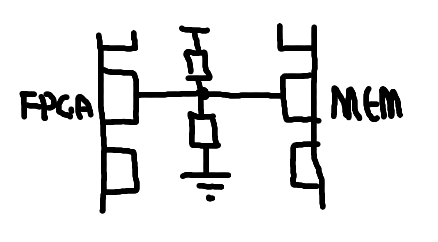
\includegraphics[width=\linewidth]{images/async_fifo.eps}
\caption[DDR Termination]{Termination scheme used to prevent
reflections/overshoot/undershoot.}
\end{center}
\end{figure}

\subsubsection{EMI}
EMI is proportional to wire height above ground
plane\cite{HighSpeedDigitalDesign}

\subsubsection{Crosstalk}
A trace a distance above the ground plane creates a loop, due to capacitance
and the ground return current. When current in this loop changes, magnetic flux
through the loop changes and this can couple with another such loop, inducing
a voltage, and this is called crosstalk.

\begin{figure}
\begin{center}
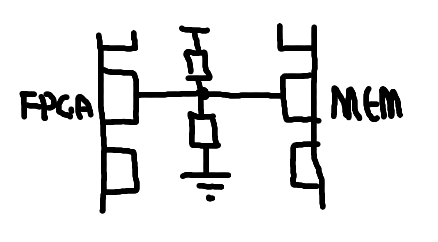
\includegraphics[width=\linewidth]{images/async_fifo.eps}
\caption{Crosstalk which is caused by magnetic coupling.}
\end{center}
\end{figure}


Include schematics as appendices and photos in here.


\subsection{Other Off-board Conections}

\subsubsection{JTAG Interface}


